\chapter{Cyclic Groups}

\section{Introduction}

For every positive integer $n$, we consider the integers modulo $n$. 

\begin{example}
    For $n = 3$, we have the multiplication table:

    \begin{minipage}[h]{0.45\linewidth} \begin{center}
        \begin{tabular}{c|c|c|c}
            $+$ & 0 & 1 & 2 \\ \hline
            0   & 0 & 1 & 2 \\ \hline
            1   & 1 & 2 & 0 \\ \hline
            2   & 2 & 0 & 1
        \end{tabular}
    \end{center} \end{minipage}
    \begin{minipage}[h]{0.45\linewidth} \begin{center}
        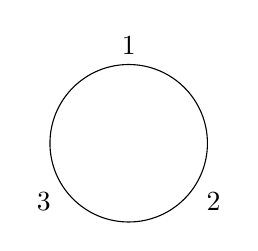
\begin{tikzpicture}
            \draw (0, 0) circle (1);
            
            \node[above] (1) at (0, 1) {1};
            \node[below right] (2) at (0.866, -0.5) {2};
            \node[below left] (3) at (-0.866, -0.5) {3};

            % Arc from 1 to 2, 2 to 3, 3 to 1, with text $+1$ on each arc
            % TODO
        \end{tikzpicture}
    \end{center} \end{minipage}

    Similarly, for $n = 4$, we have the multiplication table:

    \begin{table}[ht!]
        \centering
        \begin{tabular}{c|c|c|c|c}
            $+$ & 0 & 1 & 2 & 3 \\ \hline
            0   & 0 & 1 & 2 & 3 \\ \hline
            1   & 1 & 2 & 3 & 0 \\ \hline
            2   & 2 & 3 & 0 & 1 \\ \hline
            3   & 3 & 0 & 1 & 2
        \end{tabular}
    \end{table}
\end{example}

\begin{definition}[Cuclic Group]\index{Cyclic Group}\label{def:cyclic-group}
    Let $n$ be a positive integer. A \term{cyclic group} of order $n$ is one that admits a generator of order $n$. \[
        C_n = \{ 0, 1, \dots, n - 1 \}
    \]
\end{definition}

\begin{definition}[Generator]\index{Generator}\label{def:generator}
    A \term{generator} of a group $G$ is an element $g \in G$ such that every element of $G$ can be written as a power of $g$.
\end{definition}

The group of integers modulo $n$ is called the \term{cyclic group of order $n$} and is denoted by $C_n$ or $\Z/n\Z$.

\begin{example}
    The integers $\Z$ form a cyclic group under addition. \[ 
        \cdots \xrightarrow{+1} -2 \xrightarrow{+1} -1 \xrightarrow{+1} 0 \xrightarrow{+1} 1 \xrightarrow{+1} 2 \xrightarrow{+1} \cdots 
    \]
\end{example}

Given a group $G$ and an element $g \in G$, we produce \[
    \underbrace{\left\{ \dots, g^{-2}, g^{-1}, 1 = g^0, g, g^2, g^3, \dots \right\}}_{\langle g \rangle} \subseteq G
\]

\begin{proposition}\label{prop:order-of-cyclic-group}
    Let $G$ be a group and $g \in G$. 

    \begin{listo}
        \item The set of powers of $g$, \[
            \left\{ g^m \mid m \in \Z \right\}
        \] is a subgroup of $G$ (denoted by $\langle g \rangle$).

        \item $g$ has order $m$ if and only if $\langle g \rangle$ is isomorphic to $C_m$.
        
        \item $g$ has no order if and only if $\langle g \rangle$ is isomorphic to $\Z$.
    \end{listo}
\end{proposition}

\begin{proof}(Proposition \ref{prop:order-of-cyclic-group}.1)
    WTS $\langle g \rangle$ is a subgroup of $G$.

    \begin{listu}
        \item \textbf{Associativity} follows from that of $G$. 

        \item \textbf{Identity} is a power of $g$, namely, $g^0 = 1$.

        \item Each element has an \textbf{inverse}, indeed, the inverse of $g^n$ is $g^{-n}$ which is also a power. 

        \item \textbf{Closed} under the operation \[
            g^n \cdot g^m = g^{n + m}
        \] which is also a power. 
    \end{listu}
\end{proof}

\begin{proof}(Proposition \ref{prop:order-of-cyclic-group}.2)
    WTS $g$ has order $m$ if and only if $\langle g \rangle \cong C_m$.

    If $G$ has order $m$, \[
        1, g, g^2, \dots, g^{m - 1}
    \] are distinct.

    Define $\Phi: C_m \to \langle g \rangle$ by $\Phi(k) = g^k$.

    This is well defined if $a \equiv b \pmod{m}$, then $a = b + mt$ for some $t \in \Z$. \[
        g^a = g^{b + mt} = g^b \cdot g^{mt} = g^b \cdot (g^m)^t = g^b \cdot 1^t = g^b
    \] 

    It is an homomorphism, indeed, \[
        \Phi(a + b) = g^{a + b} = g^a \cdot g^b = \Phi(a) \cdot \Phi(b)
    \]

    \begin{listu}
        \item \textbf{Injectivity}
        
        If $\Phi(a) = \Phi(b)$, then $g^a = g^b$, so $g^{a - b} = 1$.

        We can pick $a, b \in \{ 0, 1, \dots, m - 1 \}$. We can also suppose $a \ge b$, thus \[
            0 \le a - b \le m - 1
        \]

        Then $g^{a - b} = 1$ implies $a - b = 0$, for owtherwise $g$ has order smaller than $m$. 

        Thus, $a = b$, so $\Phi$ is injective.

        \item \textbf{Surjectivity}

        By assumption \[
            \langle h \rangle = \{ g^0, g^1, \dots, g^{m - 1} \}
        \]

        Since by definition \[
            \Phi(k) = g^k,
        \] by taking $k = 0, 1, \dots, m - 1$ we produce all elements of $\langle g \rangle$.

        Thus, $\Phi$ is surjective.
    \end{listu}

    We conclude that $\Phi$ is an isomorphism.
\end{proof}

\begin{example}
    Consider $C_6 = \{ 0, 1, 2, 3, 4, 5 \}$.

    The cyclic groups the elements generate are
    \begin{listu}
        \item $0$ generates $\{ 0 \} \equiv C_1$.
        \item $1$ and $5$ generate $\equiv C_6$, $C_6 = \langle 1 \rangle = \langle 5 \rangle$.
        \item $\langle 2 \rangle = \{ 0, 2, 4\} = \langle 4 \rangle \cong C_3$. 
        \item $\langle 3 \rangle = \{ 0, 3 \} \cong C_2$.
    \end{listu}
\end{example}

\begin{example}
    We have already seen in a previous example what happens. The cyclic subgroups are

    \begin{listu}
        \item $\langle 1 \rangle = \{ \id \} = C_1$.
        \item $\langle (1, 2) \rangle = \{ \id, \langle (1, 2) \rangle \} = C_2$
        \item $\langle (1, 3) \rangle = \{ \id, \langle (1, 3) \rangle \} = C_2$
        \item $\langle (2, 3) \rangle = \{ \id, \langle (2, 3) \rangle \} = C_2$
        \item $\langle (1, 2, 3) \rangle = \{ \id, (1, 2, 3), (1, 3, 2) \rangle \} = C_3$
    \end{listu}
\end{example}

\begin{proposition}
    Let $p$ be a prime number, and $G$ be a group of order $p$. Then $G$ is cyclic, \[
        G \cong C_p
    \]
\end{proposition}

\begin{proof}
    Let $G$ be a group of order $p$. 
    
    Since $p$ is prime, $G$ has at least two elements. Thus, there exists $g \in G$ with $g \neq e$. 

    Since $G$ is finite, $g$ must have a finite order $m$. Thus, \[
        C_m = \{ 1, g, g^2, \dots, g^{m - 1} \} \subseteq G
    \]

    Let $x \in G$ and multiply by $g$ successively by the left. \[
        x \xrightarrow{g} gx \xrightarrow{g} g^2x \xrightarrow{g} \cdots \xrightarrow{g} g^{m - 1}x \xrightarrow{g} g^mx = x
    \]

    There is no repetition earlier than $m$, since otherwise $g^ix = g^jx$ for some $0 \le i < j \le m - 1$, so $g^i = g^j$ (since $g$ has order $m$), which is a contradiction.

    Doing this, we see that $G$ decomposes into cycles of size $m$. There must be a finite number of cycles, say $k$. 

    Thus, $|G| = km$, so $p = km$. Since $p$ is prime, $k = 1$ or $m = 1$.

    However, $m \neq 1$ since $g \neq e$. Thus, $k = 1$, so $m = p$ and $G = C_p$.
\end{proof}

Let us rephrase a step. Let $x \in G$, and multiply $x$ vy every element of $C_m$. 

Doing that we have
\begin{listu}
    \item $G$ a group 
    \item $H$ a subgroup of $G$ of order $m$.
    \item $x \in G$ an element. 
\end{listu}

Multiply every element of $H$ by $x$, 

\begin{example}
    Consider $S_3 = \{ \id, (1, 2), (1, 3), (2, 3), (1, 2, 3), (1, 3, 2) \}$.

    Let $H = \{ \id, (1, 2) \}$.

    \begin{listu}
        \item $H(2, 3) = \{ 1 (2, 3), (1, 2)(2, 3) \} = \{ (2, 3), (1, 2, 3) \}$
        \item $H(1, 3) = \{ 1 (1, 3), (1, 2)(1, 3) \} = \{ (1, 3), (1, 3, 2) \}$
    \end{listu}

    These two sets are called the \term{right cosets} of $H$ in $G$.
\end{example}

\begin{definition}[Coset]\index{Coset}\label{def:coset}
    Given a group $G$ and a subgroup $H$, we define a \term{coset} of $H$ in $G$ as a set of the form 
    \begin{align*}
        Hx & = \{ hx \mid h \in H \} & (\text{\term{right coset}}) \\
        xH & = \{ xh \mid h \in H \} & (\text{\term{left coset}})
    \end{align*}

    We denote by 
    \begin{listu}
        \item $H \backslash G$ the set of right cosets of $H$ in $G$, and 
        \item $G / H$ the set of left cosets of $H$ in $G$.
    \end{listu}
\end{definition}

\begin{proposition}
    Let $G$ be a group and $h$ be a subgroup of $G$. Then 
    \begin{listo}
        \item All cosets of $H$ in $G$ have the cardinality of $H$.
        \item All left cosets are disjoint, and so are all right cosets.
    \end{listo}
\end{proposition}

\begin{proof}
    We prove the two statements. 

    \begin{listo}
        \item Multiplying by $x$ is a bijection.
        
        \item Suppose $xH \cap yH \neq \varnothing$. 
        
        Then there exists $z \in xH \cap yH$, that is, $z = xh_1 = yh_2$ for some $h_1, h_2 \in H$.
        \begin{align*}
            y^{-1} x h^1 {h_1}^{-1} & = y^{-1} y h_2 {h_1}^{-1} \\ 
            y^{-1} x                & = h_2 {h_1}^{-1} \in H
        \end{align*}
        Then, $y^{-1} x = h$ for some $h \in H$, so $x = yh \in yH$.

        But then for $x \tilde{h} \in xH$, $\begin{aligned}[t]
            x \tilde{h} & = (yh) \tilde{h} \\
                        & = y (h \tilde{h}) \in yH
        \end{aligned}$

        That is, $xH \subseteq yH$. Similarly, $yH \subseteq xH$, so $xH = yH$.
    \end{listo}
\end{proof}

\begin{theorem}[Langrange's Theorem]\index{Langrange's Theorem}\label{thm:langrange}
    Let $G$ be a finite group and $H$ be a subgroup of $G$. Then \[
        |G| = |H| \text{ divides } |G|
    \]
\end{theorem}

\begin{proof}
    $G$ is a disjoint union of cosets of $H$ in $G$.

    Say there are $k$ cosets. Then \[
        |G| = k |H| \implies H \mid G
    \]
\end{proof}

\begin{corollary}[Corollary of Proposition]\label{cor:cyclic-subgroup}
    Let $H \leq G$ be a subgroup of a finite group $G$. Then 
    \begin{listo}
        \item $xH = yH$ if and only if $y^{-1}x \in H$.
        \item $Hx = Hy$ if and only if $xy^{-1} \in H$.
    \end{listo}
\end{corollary}

\begin{example}
    $C_n$ has order $N$. $n$ has certain divisors, and $C_n$ has a generator $g$: \[
        C_n = \{ 1, g, g^2, \dots, g^{n - 1} \}
    \]

    Consider when $n = 12$. 

    $C_n = \Z / 12\Z = \{ 0, 1, 2, \dots, 11 \}$

    12 = $4 \times 3$, so the devisors are 

    \begin{table}[ht!]
        \centering
        \begin{tabular}{c|c}
            $1$  & $\{ 0 \}$ \\ \hline
            $2$  & $\{ 0, 6 \}$ \\ \hline
            $3$ & $\{ 0, 4, 8 \}$ \\ \hline
            $4$ & $\{ 0, 3, 6, 9 \}$ \\ \hline
            $6$ & $\{ 0, 2, 4, 6, 8, 10 \}$ \\ \hline
            $12$ & $\{ 0, 1, 2, \dots, 11 \}$
        \end{tabular}
    \end{table}

    $C_n$has exactly one subgroup of each order dividing $n$.

    We can construct a subgroup map. 

    \begin{figure}[ht!]
        \centering
        
        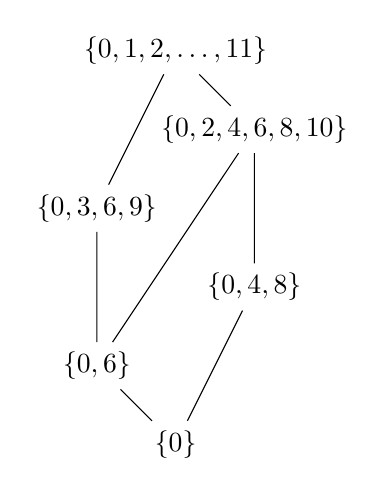
\begin{tikzpicture}
            \node (c1) at (0, 0) {$\{ 0 \}$};
            \node (c2) at (-1, 1) {$\{ 0, 6 \}$};
            \node (c3) at (1, 2) {$\{ 0, 4, 8 \}$};
            \node (c4) at (-1, 3) {$\{ 0, 3, 6, 9 \}$};
            \node (c6) at (1, 4) {$\{ 0, 2, 4, 6, 8, 10 \}$};
            \node (c12) at (0, 5) {$\{ 0, 1, 2, \dots, 11 \}$};

            \draw (c1) -- (c2) -- (c6) -- (c12);
            \draw (c1) -- (c3) -- (c6);
            \draw (c2) -- (c4) -- (c12);
        \end{tikzpicture}
    \end{figure}

    This is called the \term{Hasse diagram} of the subgroup lattice of $C_{12}$.
\end{example}